%!TEX root = ../planets-notes.tex

What do we actually measure when we observe a star? A star emits photons with a range of wavelengths over the electromagnetic spectrum.  The total emitted energy per second over all wavelengths is the star's \emph{luminosity}.  For example, the solar luminosity is $\Lsun = \val{\sci{3.86}{26}}{\unitstyle{W}}$.  A telescope collects only a small fraction of this power: if a telescope has a collecting area $\mathcal{A}$ and is a distance $d$ from the star, then it intercepts a fraction $\mathcal{A}/(4\pi d^{2})$ of the star's light.  We call $F = L/(4\pi d^{2})$ the \emph{flux}. The units of flux are $\unitstyle{W}\,\meter^{-2}$.

More specifically, $F$ is the \emph{bolometric flux}, that is, the flux over all wavelengths.  Of course, no telescope detects \emph{all} wavelengths of light. Many wavebands, e.g., UV, X-ray, and infrared, do not even penetrate the Earth's atmosphere.  Moreover, detectors (photographic plates or CCD's) are not uniformly efficient at converting photons into a signal.

In order to have a common standard, (optical) astronomers use \emph{filters}, which transmit light only in certain wavelength bands. In this context, the flux refers to the power per area carried by light with wavelengths in that band.  For historical reasons, astronomers define \emph{magnitudes}, which are a relative logarithmic\sidenote{In these notes, $\lg\equiv\log_{10}$ and $\ln\equiv\log_{e}$.} scale for fluxes.  The difference in magnitude between two stars is defined by
\begin{equation}\label{e.magnitude-def}
	m_{1} - m_{2} = -2.5\lg\left(\frac{F_{1}}{F_{2}}\right)
\end{equation}
where the magnitudes $m_{1}$, $m_{2}$ and fluxes $F_{1}$, $F_{2}$ refer to light that has been passed through a particular filter.

\begin{margintable}
\label{t.ubvr}\caption{Selected common filters about the range of visible wavelengths \citep{Binney1998Galactic-Astron}.  Here ``FWHM'' means ``Full width at half-maximum.''}
\begin{tabular}{lrr}
\hline
Filter & $\lambda_{\mathrm{eff}}/\nano\meter$ & FWHM/nm \\
\hline\hline
U & 365 &  66\\
B & 445 &  94\\
V & 551 &  88\\
R & 658 & 138\\
\hline
\end{tabular}
\end{margintable}

Note that magnitudes are defined as the ratio of two fluxes. This is very useful when comparing the relative brightness of two stars; unfortunately it makes conversion to a physical unit ($\unitstyle{W}\usk\meter^{-2}\usk\nano\meter^{-1}$) non-trivial.  The magnitude scales are typically defined so that the star Vega has $U=B=V=\ldots=0$.\sidenote{But for historical reasons, $V(\textrm{Vega}) = +0.04.$}


\newpage
\begin{exercisebox}[Relation between magnitude and flux]
\begin{enumerate} 
\item Suppose we have two identical stars, A and B. Star A is twice as far away as star B. What is $m_{A} - m_{B}$?
\item Suppose a star's luminosity changes by a tiny amount $\delta$.  What is the corresponding change in that stars' magnitude?
\end{enumerate}
\end{exercisebox}

\newthought{If we take a ratio of two magnitudes using different filters from a single star,} then we have a rough measure of the star's color.  This ratio is called a \emph{color index}.  For example, 
\[ B - V \equiv m_{B} - m_{V} = -2.5\lg\frac{F_{B}}{F_{V}} \]
gives a measure for how blue the star's spectrum appears.

\begin{exercisebox}[The $B-V$ index]
Which has the larger $B-V$ index: a red star, like Betelgeuse, or a blue-white star, like Rigel?
\end{exercisebox}

\newthought{Two stars with the same apparent brightness} may have very different intrinsic brightnesses: one may be very dim and nearby, the other very luminous and faraway.  To compare intrinsic brightness, we need to correct for the distance to the star\sidenote{This assumes we \emph{know} the distance, which can be difficult!}.  We define the \emph{distance modulus} as the difference in magnitude between a given star and the magnitude it would have if it were at a distance of \val{10}{\parsec}:
\begin{eqnarray*}
 \mathrm{DM} \equiv m - m(\val{10}{\parsec}) &=& -2.5\lg\left[\frac{L}{4\pi d^{2}} \frac{4\pi (\val{10}{\parsec})^{2}}{L}\right] \\
 	&=& -2.5\lg\left(\frac{\val{10}{\parsec}}{d}\right)^{2} \\
	&=& 5\lg\left(\frac{d}{\parsec}\right) - 5.
\end{eqnarray*}
The magnitude that the star would have if it were at \val{10}{\parsec} distance is called its \emph{absolute magnitude}, $M \equiv m - \mathrm{DM}$.

\section{Light is a wave}

\begin{marginfigure}
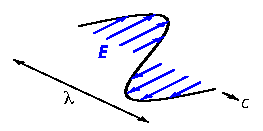
\includegraphics[width=\linewidth]{light-wave}
\caption[The electric force in a light wave]{Schematic of the electric force (blue arrows) for a wave traveling towards us at speed $c$ with wavelength $\lambda$.}
\label{f.light-wave}
\end{marginfigure}
Charges feel an electric force.
When we detect light, what happens at the atomic level is that the charges in our detector (antenna, CCD, eye) feel an electric force that oscillates with frequency $\nu$. If we could set up a grid of detectors and measure the electric force per unit charge, we would notice a sinusoidal pattern traveling at speed\sidenote{This velocity is exact; the meter is defined in terms of the speed of light.} $c = \val{299\,792\,458}{\meter/\second}$ with a wavelength $\lambda = c/\nu$.  We call this force per charge the electric field $\bvec{E}(\bvec{x},t)$. The \emph{intensity} of the light at our detector is proportional to $|\bvec{E}|^{2}$.

In situations in which the wavelength is small (relative to the system in question), light propagates along \emph{rays}.  The rule for propagation is known as \emph{Fermat's principle:} the path is that for which the propagation time is minimized. To illustrate this, we shall use it to derive the laws for reflection and refraction.

Consider light reflecting from a mirror as shown in the top panel of Figure~\ref{f.reflection-and-snell}. The time for light to propagate from source to observer is
\[	\tau = \frac{1}{c}\left[\sqrt{h_{s}^{2}+x^{2}} + \sqrt{h_{o}^{2} + (w-x)^{2}}\right]. \]
To minimize the path length, we compute $\dif\tau/\dif x$ and set it to zero,
\[
	0 = \DD{\tau}{x} = \frac{1}{c}\left[\frac{x}{\sqrt{h_{s}^{2}+x^{2}}} 
	- \frac{w-x}{\sqrt{h_{o}^{2} + (w-x)^{2}}}\right] = \frac{1}{c}\left[\sin i - \sin r\right].
\]
Hence the light travels such that $i = r$: the angles of incidence and reflection are equal.

\begin{marginfigure}
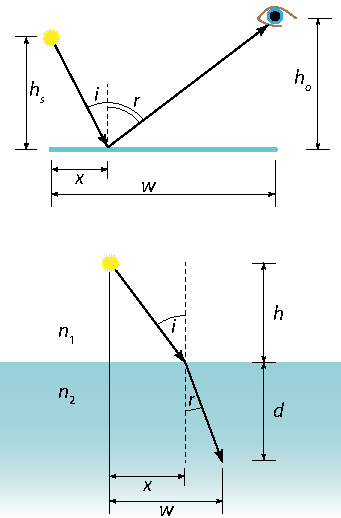
\includegraphics[width=\linewidth]{reflection-and-snell-AST208}
\caption{Top: reflection of light from a surface. Bottom: refraction of light as it passes from a medium with index $n_{1}$ into a medium with index $n_{2}$.
\label{f.reflection-and-snell}}
\end{marginfigure}

For a second example, consider the passage of light from one medium to another, as depicted in the bottom panel of Figure~\ref{f.reflection-and-snell}.  The interaction of matter with the oscillating electric field causes the light to travel at a speed $c/n$, where $n$ is called the \emph{index of refraction} and is a property of the material. For the situation in Fig.~\ref{f.reflection-and-snell}, the propagation time is
\[
	\tau = \frac{n_{1}}{c}\sqrt{h^{2}+x^{2}} + \frac{n_{2}}{c}\sqrt{d^{2} + (w-x)^{2}};
\]
minimizing the propagation time with respect to $x$ gives
\[
	0 = \frac{n_{1}}{c}\frac{x}{\sqrt{h^{2}+x^{2}}} - \frac{n_{2}}{c} \frac{w-x}{\sqrt{d^{2} + (w-x)^{2}}} = \frac{1}{c}\left[ n_{1}\sin i - n_{2} \sin r \right].
\]
This result, $n_{1}\sin i = n_{2}\sin r$, is also known as \emph{Snell's law}.

\begin{marginfigure}[5em]
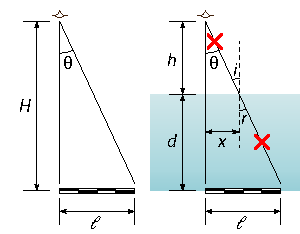
\includegraphics[width=\linewidth]{magnification-in-water}
\caption{Change in angular size of an object in water.
\label{f.magnification-in-water}}
\end{marginfigure}
\begin{exercisebox}[Magnification of an object in water]
A small stick of length $\ell$ is placed on the bottom of an empty swimming pool as shown in Fig.~\ref{f.magnification-in-water}; when you look down on the stick from a height $H$ above the bottom of the pool, the stick subtends an angle $\tan\theta = \ell/H$.  The pool is then filled with water ($n=4/3$) to a depth $d$.  Because of refraction, the stick will appear to subtend a different angle $\theta'$.  Correct the right hand diagram of Fig.~\ref{f.magnification-in-water} to show how the light ray propagates from the ends of the stick to your eye.  Is $\theta'$ larger or smaller than $\theta$---is the image of the stick magnified or reduced?  For the case $\ell \ll H$, so that $\theta \ll 1$, use the small angle expansions to derive an expression $\theta' = 
\theta \mathcal{M}$, where $\mathcal{M}$ depends on $h$, $d$, and $n$.
\end{exercisebox}

\section{Diffraction}

A telescope makes an image by focusing the incoming rays of light onto a detector.
Suppose we are at a fixed point and the wave is propagating past us.  In general we would observe an electric field amplitude of the form 
\[ E(t) = A_{0}\cos\left(2\pi \nu t \right)  + B_{0}\sin\left(2\pi \nu t \right) \]
where $\nu = c/\lambda$ is the frequency.  Let's check this: in going from $t=0$ to $t=T=1/\nu$, the period of the wave, the argument of the cosine and sine goes from $0$ to $2\pi$, which is one oscillation.  To find the net intensity $I$ from a number of waves, we sum the amplitudes to get the net electric field $\bvec{E}$ and then take the square $|\bvec{E}|^{2}$.

Now imagine the electromagnetic wave incident on our telescope. The source is very distant, so the wavefront (a surface of constant phase) is a plane---think of sheets of paper moving downward onto the telescope.  To make an image, the telescope focuses the incident radiation to a point on the detector. There is a limit, however, to how sharply the image can be focused.  Let's look at a small angle $\theta$ away from the axis.  Then the wavefront is incident on the telescope as shown in Figure~\ref{f.diffraction}. To keep the math tractable, we'll make our telescope opening one-dimensional and we'll break it into a $N+1$ little detectors spaced a distance $d = D/N$ apart.

\begin{figure}[hb]
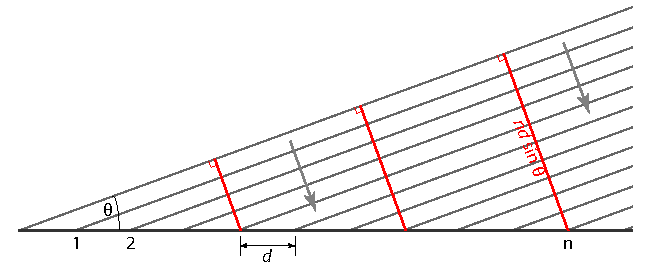
\includegraphics[width=\linewidth]{diffraction}
\caption[A plane wave incident on a detector]{Schematic of a plane wave incident at angle $\theta$ on a detector.}
\label{f.diffraction}
\end{figure}

Because of the angle, the light travels an extra distance $d\sin\theta$ to reach detector 1, $2d\sin\theta$ to reach detector 2, and so on.  As a result, if the phase at the first detector (number 0) is $\chi$, the phase at detector 1 is $\chi + 2\pi d\sin\theta/\lambda$, at detector 2,  $\chi + 4\pi d\sin\theta/\lambda$, and so on.  When we combine the signals from these detectors, the amplitude of the electric field will have the form
\begin{eqnarray*}
E &=& A_{0}\left[\cos\chi + \cos\left(\chi + 2\pi\frac{d\sin\theta}{\lambda}\right)
	+ \cos\left(\chi + 2\pi\frac{2d\sin\theta}{\lambda}\right) + \right.\\
	&&	+ \left.\cos\left(\chi + 2\pi\frac{3d\sin\theta}{\lambda}\right) + \ldots 
	+ \cos\left(\chi + 2\pi\frac{Nd\sin\theta}{\lambda}\right)\right]\\
	&& + B_{0}\left[ \sin\chi + \sin\left(\chi + 2\pi\frac{d\sin\theta}{\lambda}\right) 
		+ \ldots + \sin\left(\chi+2\pi\frac{Nd\sin\theta}{\lambda}\right)\right].
\end{eqnarray*}
When $\theta \to 0$, the amplitude goes to $E \to (N+1)\left[A_{0}\cos\chi + B_{0}\sin\chi\right]$, and so the brightness $I(\theta\to 0) = |E|^{2}$ is a very large number.  That's good: the light from the star is focused to a point. Now, how large does $\theta$ have to be before $E$ goes to zero?

To find this, let's first set $\chi = 0$ to keep things simple. There are a number of ways to find the sum; a particularly easy way is to recognize that this sum over cosines looks like adding up the $x$-component of vectors, and the sum over the sines looks like adding the $y$-component of vectors.  We add the vectors by placing them nose-to-tail as shown in Fig.~\ref{f.vector-addition}.  The net amplitude is then $A_{0}$ times the $x$-component of the red vector, plus $B_{0}$ times the $y$-component of the red vector.  Clearly if we want both the sum over sines and over cosines to vanish, we need the vectors to make a complete circle.

\begin{marginfigure}
\centering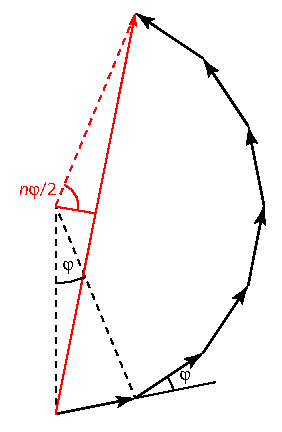
\includegraphics[width=0.8\linewidth]{vector-addition}
\caption[Addition of vectors with phase differences]{Addition of a series of vectors with a phase difference $\phi$.}
\label{f.vector-addition}
\end{marginfigure}

In this addition, each vector has length 1. If $N+1$ is large, then the circumference of the circle is approximately $(N+1) = 2\pi r$.  For small $\phi = (2\pi d/\lambda)\sin\theta$, the radius of the circle is $r \approx 1/\phi$.  Hence the condition for our vectors to sum to zero becomes
\[ N+1 = \frac{2\pi}{\phi} = \frac{2\pi\lambda}{2\pi d\sin\theta} \]
Now, we assume that $N \gg 1$, so that $(N+1)d \approx Nd = D$, the diameter of our telescope's aperture.  Then, the brightness falls to zero an angle
\[ \sin\theta \approx \theta \approx\lambda/D\]
away from the center of the star's image.

The full form of the intensity as a function of angle from the beam axis is,
\begin{equation}\label{e.intensity-diffraction}
I = I_{0}\left[\frac{\sin\left(\pi D/\lambda\,\sin\theta\right)}{\sin\left(\pi d/\lambda\,\sin\theta\right)}\right]^{2}.
\end{equation}

\begin{exercisebox}[Diffraction of image of a point source]
Write a \code{Python} function that computes eq.~(\ref{e.intensity-diffraction}) for different values of $N$ and $D/\lambda$.  Plot $I/(I_{0}n^{2})$ against $\theta\lambda/D$.  Describe your findings.
\end{exercisebox}

The wave nature of light places a limitation on the \emph{resolving power} of a telescope, defined as the   angular separation for which two point sources can be distinguished.  Two point-like objects separated by an angular distance $\lesssim \lambda/D$ will have their images smeared into one.

\begin{exercisebox}[Resolving power of various instruments]
What is the resolving power of the \emph{Hubble Space Telescope} ($D=\val{2.4}{\meter}$) and the Keck telescope ($D=\val{10}{\meter}$) at a wavelength $\lambda = \val{570}{\nano\meter}$? Estimate the angular resolution of the human eye at that wavelength. What is the resolving power of the Arecibo radio telescope ($D = \val{305}{\meter}$) at a frequency of \val{3}{\Giga\Hz}?
\end{exercisebox}

For ground-based telescopes, an even more severe limitation is the refraction of light by the atmosphere. The atmosphere is turbulent, and the swirling eddies contain variations in density that change the refractive index and distort the wavefront.  This distortion smears the image over an angular scale that is typically larger than $1''$.

\begin{exercisebox}[Angular size of star, planet]
What is the angular size of a solar-sized star ($\Rsun = \val{\sci{6.96}{5}}{\kilo\meter}$) at a distance of $\val{1}{\parsec}$?  What is the angular size of Mars ($R_{\mars} = \val{3\,390}{\kilo\meter}$) at a distance of $\val{0.5}{\AU}$?  How would the difference in angular size affect the appearance of these two objects?
\end{exercisebox}

\newthought{In addition to distorting the wavefront, the air also attenuates the brightness of the light.} The amount of attenuation depends on the column, that is, the mass per unit area of air along the line of sight, which in turn depends on the viewing angle (Fig.~\ref{f.airmass}).

\begin{marginfigure}
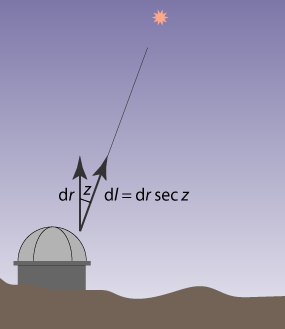
\includegraphics[width=\linewidth]{airmass}
\caption[Illustration of airmass]{Illustration of the greater column of atmosphere (\emph{airmass}) that the light from a star an angle $z$ from the zenith must traverse.}
\label{f.airmass}
\end{marginfigure}

Astronomers define the \emph{airmass} $m$ as a function of zenith angle $z$ by
\[
	\textrm{air mass} = \frac{\int\rho(r)\,\dif \ell}{\int\rho(r)\,\dif r}
\]
where $\ell$ is along the line of sight to the star.  For a planar atmosphere, $\dif\ell = \dif r/\cos z = \sec z\,\dif r$, and so the airmass is just $\sec z$.  The dimming of the star is proportional to $\exp\left[-\int\rho(r)\,\dif\ell\right]$, and therefore the magnitude of a star at zenith angle $z$ varies as
\[ m(z) = k \sec z + c, \]
where $k$ and $c$ are constants.  By measuring the apparent brightness of the star at several different zenith angles, astronomers can empirically determine these constants.
